\documentclass[12pt]{article}

\usepackage[T1]{fontenc}
\usepackage[margin=1in]{geometry}
\usepackage{booktabs}
\usepackage{graphicx}
\usepackage{caption}
\usepackage{subcaption}
\usepackage{float}
\usepackage{hyperref}
\usepackage{setspace}
\usepackage{placeins}

\graphicspath{{../output/}{../}}
\onehalfspacing

\title{Plugged In or Crowded Out? Replicating and Extending Evidence on EV Charging Stations and Local Business Activity}
\author{Arik Lemon \and Kevin Sheng}
\date{\today}

\begin{document}

\maketitle

\begin{abstract}
This replication studies whether electric vehicle charging stations (EVCS) affect nearby business activity. The analysis replicates direct EVCS spillover estimates and extends the design to same-sector spatial competition. Narrow two-way fixed effects estimates are positive for all points of interest (POIs), while broader stacked own-port estimates are weaker and more mixed, with the clearest negative associations for DC fast charging exposure. Spatial competition estimates show that all-port and Level 2 competitor exposure are essentially null, while DC fast exposure at nearby same-sector competitors is negatively associated with customer counts and spending. Pretrend and placebo diagnostics motivate cautious causal language, so the evidence is framed as robust associations rather than definitive causal effects.
\end{abstract}

\section{Introduction}
Electric vehicle charging infrastructure is increasingly visible in local retail and service environments. Electric vehicle charging stations (EVCS) are usually discussed as transportation and climate infrastructure, but they may also affect nearby businesses. When drivers stop to charge, they may visit restaurants, shops, hotels, or other local establishments nearby. If this behavior is common, EVCS could generate local economic spillovers in addition to supporting electric vehicle adoption.

This report replicates and extends Zheng et al. (2024), which studies the effect of EVCS openings on business activity in California. The original paper finds that new charging stations are associated with higher customer visits and spending at nearby points of interest (POIs), especially for businesses close to the station. Utilizing the same underlying data sources as the original study, our project is conducted as a scoped replication. We use the available replication code and reconstructed data pipeline to evaluate whether the paper’s main patterns hold under our data scope.

Our analysis has three parts. First, we conduct a narrow replication of the paper’s main two-way fixed effects design, focusing on businesses within 500 meters of newly opened EVCS during 2019 and 2021-2023. Second, we broaden the replication window through January 2026 and use staggered-adoption and stacked specifications to examine whether the relationship changes over a longer period. Third, we add a spatial competition extension, asking whether EVCS exposure at nearby same-sector competitors is associated with reduced activity at focal businesses.

Overall, the project treats replication as both a validation exercise and a robustness check. Rather than requiring exact numerical equality with the original paper, we focus on whether the estimated direction, magnitude, and interpretation of EVCS-business spillovers remain plausible when the sample, window, and empirical design are made explicit.

%This paper asks whether EV charging stations affect nearby business activity. The core empirical question is whether exposure to active EVCS ports changes customer visits and spending at nearby consumer-facing establishments.

The contribution is twofold. First, the paper replicates direct EVCS spillover estimates using narrow windows that match the original empirical setting. Second, it extends the design to same-sector spatial competition by asking whether chargers located at nearby competitors are associated with changes in activity at focal businesses without chargers.

%The results differ across designs. Narrow two-way fixed effects (TWFE) estimates are positive for all POIs. Broader stacked own-port estimates are negative, especially for DC fast chargers. Spatial competition estimates show robust negative associations with DC fast competitor exposure, with the clearest subgroup evidence among restaurants. Because pretrend and placebo diagnostics are statistically significant in the stacked designs, the findings are interpreted cautiously.

\section{Data and Variables}
Our analysis combines business activity data, electric vehicle charging station records, demographic controls, and built-environment measures to study how EV charging infrastructure is associated with nearby local economic activity. Our replication is conducted as a scoped replication rather than an exact reconstruction of the published analysis sample, using Python instead of R. The data pipeline follows the paper’s core design, but the extension restricts attention to consumer-facing businesses in a clearly defined local-business context. This makes the exercise useful both as a replication attempt and as a robustness check for whether the paper’s main patterns persist under a more transparent reconstructed sample.

The main business outcomes come from SafeGraph point-of-interest data. We use monthly measures of customer visits and customer spending for California business establishments. The two primary dependent variables are the natural log of one plus monthly customer counts, lcus, and the natural log of one plus monthly total customer spending, lspend. Additional outcomes are used in auxiliary analyses, including customer counts by income group, average customer income, median dwell time, and median distance from home where relevant foot-traffic data are available.

Charging station information comes from the U.S. Department of Energy Alternative Fuels Data Center. For each public EV charging station, the data include location, opening date, number of charging ports, and charger type. The main treatment variable measures active charging-port exposure near a business. Specifically, port\_treat is the number of active EV charging ports within 500 meters of a POI in a given month. We also separate this exposure into Level 2 ports and DC fast charging ports, allowing the analysis to test whether slower destination-style charging and faster charging infrastructure have different associations with business activity. For distance heterogeneity, port exposure is also divided into 100-meter bins from 0 to 500 meters.

For the narrow replication, we follow the original study windows as closely as possible: January to December 2019, and January 2021 to June 2023, with January 2021 serving as the baseline outcome month and EVCS treatment beginning in February 2021. Propensity-score matched panels are constructed separately for each period and for all-region versus disadvantaged-community samples. Matching is based on POI category and covariates including built-environment characteristics, tract-level demographics, county-level EV adoption, and baseline POI outcomes.

For the broad replication, we extend the second period through January 2026. This broader window allows us to examine whether the short-run relationships in the narrow replication persist as charging infrastructure becomes more widespread and treatment timing becomes more staggered. The broad analysis uses the same core outcomes and direct EVCS exposure variables, but it is organized around staggered-adoption and stacked event-window designs rather than only the original two-way fixed effects specification.

Finally, the report includes a spatial competition extension. In that part of the analysis, the focal unit is a non-EVCS business, and treatment is defined as charging-port exposure at nearby same-sector competitors. The main competitor radius is 1,000 meters, which is intentionally larger than the 500-meter direct-exposure radius. These variables are labeled as competitor port exposure, with separate measures for all ports, Level 2 ports, and DC fast ports. This extension shifts the question from whether EVCS increase activity at nearby businesses to whether charger-equipped competitors may draw activity away from otherwise similar nearby establishments.

For the extension, the POI sample is restricted to consumer-facing establishments in NAICS sectors 44, 45, 71, and 72, covering retail trade, arts/entertainment/recreation, and accommodation/food services. In this context, a POI must have at least one other target-category business within 500 meters. This choice narrows the analysis to businesses plausibly located in commercial areas where EVCS-related spillovers are meaningful, but it also means that our sample differs from the published paper’s exact sample in this setting. Underprivileged-community status is measured using California Energy Commission and Justice40 disadvantaged or low-income community geography, rather than only using income proxies.

%The analysis combines Dewey spend and foot-traffic measures, National Renewable Energy Laboratory Alternative Fuels Data Center EVCS records, Census and American Community Survey covariates, and built-environment controls. The sample focuses on consumer-facing target NAICS sectors in a local-business context.

%Two time windows are used. The narrow replication window covers 2019 and February 2021 through June 2023. The broad window covers 2019 and February 2021 through January 2026. Direct exposure is measured as active EVCS ports within 500 meters of a POI, split into all ports, Level 2 ports, and DC fast ports. Spatial competition exposure measures active charger ports at nearby same-sector competitors, with a 1000 meter radius used as the main specification.

\section{Econometric Specifications}

We estimate the relationship between EV charging station exposure and nearby business activity using several related panel-data specifications. The narrow replication follows the original paper most closely, while the broad replication and spatial competition models extend the design to longer windows and alternative treatment definitions.

We estimate this model separately for 2019 and 2021-2023, and separately for all POIs and disadvantaged-community POIs. We also estimate variants that split treatment by distance bin and charger type. The distance specification replaces the main treatment variable with active port counts in 100-meter bins between 0 and 500 meters. The charger-type specification separates exposure into Level 2 ports and DC fast charging ports.

For the broad replication, we extend the second study window through January 2026. Because treatment timing is staggered across POIs, we supplement the TWFE approach with staggered-adoption estimators. First, we use the Callaway-Sant'Anna estimator that compares treated POIs to not-yet-treated POIs by treatment cohort and month. This provides a timing-based diagnostic that is less dependent on the homogeneous-treatment-effect assumptions of TWFE.

Our preferred broad specification is a stacked event-window regression. For each treatment cohort, we construct a local panel around the EVCS opening date using a six-month pre-treatment window and a twelve-month post-treatment window. We then stack these cohort-specific panels and estimate treatment effects with stack-specific fixed effects. This design compares newly treated POIs to clean controls observed in the same relative time window, reducing contamination from already-treated units.

For the spatial competition extension, we use a similar stacked design but redefine treatment. Instead of measuring a POI’s own direct exposure to EVCS within 500 meters, we measure charger exposure at nearby same-sector competitors. The main competition radius is 1,000 meters, which keeps it distinct from the direct 500-meter EVCS exposure definition. This specification tests whether charging infrastructure at competing businesses is associated with changes in customer counts or spending at nearby focal POIs.

Across all specifications, the coefficients are interpreted as approximate percentage changes because the dependent variables are logged. Our replication uses a reconstructed sample from the same original data sources found in the original paper, therefore we interpret the estimates as evidence on robustness and direction rather than as exact numerical reproductions.

%The narrow replication uses a TWFE specification with POI fixed effects and county-month fixed effects, with standard errors clustered by POI. The broad timing diagnostic uses a Callaway-Sant'Anna estimator with not-yet-treated controls.

%The preferred broad and spatial specifications use stacked near-treatment regressions. These models define cohort stacks around treatment timing, use clean controls, include a 6-month pre-window and 12-month post-window, and absorb stack-specific POI and county-month fixed effects. To keep estimation feasible and comparable across specifications, the stacked designs use a 10,000-control cap.

%The estimates are interpreted as robust associations. Significant pretrend and placebo terms limit strong causal claims, especially in the broader staggered and spatial competition designs.

\section{Narrow Replication Results}

The narrow replication estimates the original two-way fixed effects specification for the 2019 and 2021-2023 study windows. Overall, the results recover the main qualitative finding of the original paper: EVCS exposure is positively associated with nearby business activity. In the all-region sample, an additional active charging port within 500 meters is associated with a 0.179\% increase in customer counts and a 0.235\% increase in spending in 2019. For 2021-2023, the corresponding estimates are 0.123\% for customer counts and 0.157\% for spending. All four estimates are statistically significant.

The disadvantaged-community estimates are also positive, though less consistently significant. In 2019, the estimated effects are 0.166\% for customer counts and 0.269\% for spending, but neither estimate is statistically significant at conventional levels. In 2021-2023, the customer-count estimate is 0.115\% and marginally significant, while the spending estimate is 0.169\% and statistically significant. These results suggest that EVCS exposure may also benefit businesses in disadvantaged areas, but the evidence is weaker and more sensitive to the reconstructed sample than in the all-region estimates.

The distance results generally support the idea that proximity matters. For the 2021-2023 all-region sample, the largest effects occur within 0-100 meters of an EVCS: 0.579\% for customer counts and 0.755\% for spending. Effects at farther distance bins are smaller and less consistent. The 2019 pattern is positive across most bins but less monotonic, suggesting that the spatial gradient is present but not perfectly smooth in our reconstructed data.

Charger-type results show that DC fast chargers play a particularly important role in this replication. In 2019, DC fast port exposure is positive and statistically significant for both customer counts and spending, while Level 2 exposure is close to zero. In 2021-2023, both Level 2 and DC fast chargers are positively associated with all-region business activity, but DC fast chargers have the larger estimated effect. This differs somewhat from the original paper’s interpretation, so we treat the charger-type results as suggestive rather than definitive.

The income-group results are broadly consistent with the paper’s finding that EVCS attract customers across income groups, with stronger effects among higher-income customers in the later period. In 2021-2023, the largest all-region customer-count effects appear for the \$75-100k, \$100-150k, and above \$150k groups. The other-outcome analysis also shows that EVCS exposure is associated with higher average customer income in 2021-2023, while the 2019 estimate is close to zero. Auxiliary foot-traffic outcomes are more sparsely observed. In the 2021-2023 all-region and disadvantaged-community samples, EVCS exposure is associated with shorter median distance from home. Median dwell-time estimates are less stable because several cells have very small sample sizes or are partially absorbed by fixed effects, so these auxiliary outcomes are interpreted as descriptive supporting evidence rather than core results.

\begin{table}[!htbp]
\centering
\caption{Table 1. Narrow TWFE estimates of EVCS exposure on nearby POI activity}
\begin{tabular}{lllllll}
\toprule
Period & Sample & Outcome & Estimate (SE), \% & 95\% CI, \% & p & N \\
\midrule
Period1 2019 & All & Customers & 0.163*** (0.039) & [0.087, 0.238] & < .001 & 126,594 \\
Period1 2019 & All & Spending & 0.204*** (0.051) & [0.103, 0.304] & < .001 & 126,594 \\
Period1 2019 & Disadvantaged & Customers & 0.002 (0.141) & [-0.274, 0.278] & .990 & 20,990 \\
Period1 2019 & Disadvantaged & Spending & 0.069 (0.195) & [-0.314, 0.451] & .726 & 20,990 \\
Period2 2021 2023 & All & Customers & 0.113*** (0.030) & [0.055, 0.170] & < .001 & 700,808 \\
Period2 2021 2023 & All & Spending & 0.158*** (0.036) & [0.088, 0.228] & < .001 & 700,808 \\
Period2 2021 2023 & Disadvantaged & Customers & 0.101 (0.075) & [-0.046, 0.248] & .177 & 94,396 \\
Period2 2021 2023 & Disadvantaged & Spending & 0.101 (0.089) & [-0.073, 0.275] & .255 & 94,396 \\
\bottomrule
\end{tabular}
\begin{minipage}{0.95\linewidth}\footnotesize\emph{Note.} Entries are log-point coefficients converted to percent units. Standard errors are clustered by POI and shown in parentheses. * p < .05, ** p < .01, *** p < .001.\end{minipage}
\end{table}


\begin{table}[!htbp]
\centering
\caption{Table 2. Narrow-replication monetary interpretation}
\begin{tabular}{lllll}
\toprule
Period & Sample & Annual spend per POI & Annual customers per POI & Annual spend within 500m \\
\midrule
Period1 2019 & All & \$6,547 & 68.1 & \$98,202 \\
Period1 2019 & Disadvantaged & \$7,458 & 67.8 & \$111,876 \\
Period2 2021 2023 & All & \$1,135 & 13.0 & \$9,084 \\
Period2 2021 2023 & Disadvantaged & \$944 & 10.4 & \$7,550 \\
\bottomrule
\end{tabular}
\begin{minipage}{0.95\linewidth}\footnotesize\emph{Note.} Monetary impacts apply the narrow TWFE spend coefficient to average pretreatment spending, average ports per EVCS, and the average number of nearby POIs used in the replication calculation.\end{minipage}
\end{table}


\begin{figure}[!htbp]
    \centering
    \begin{subfigure}{0.48\linewidth}
        \centering
        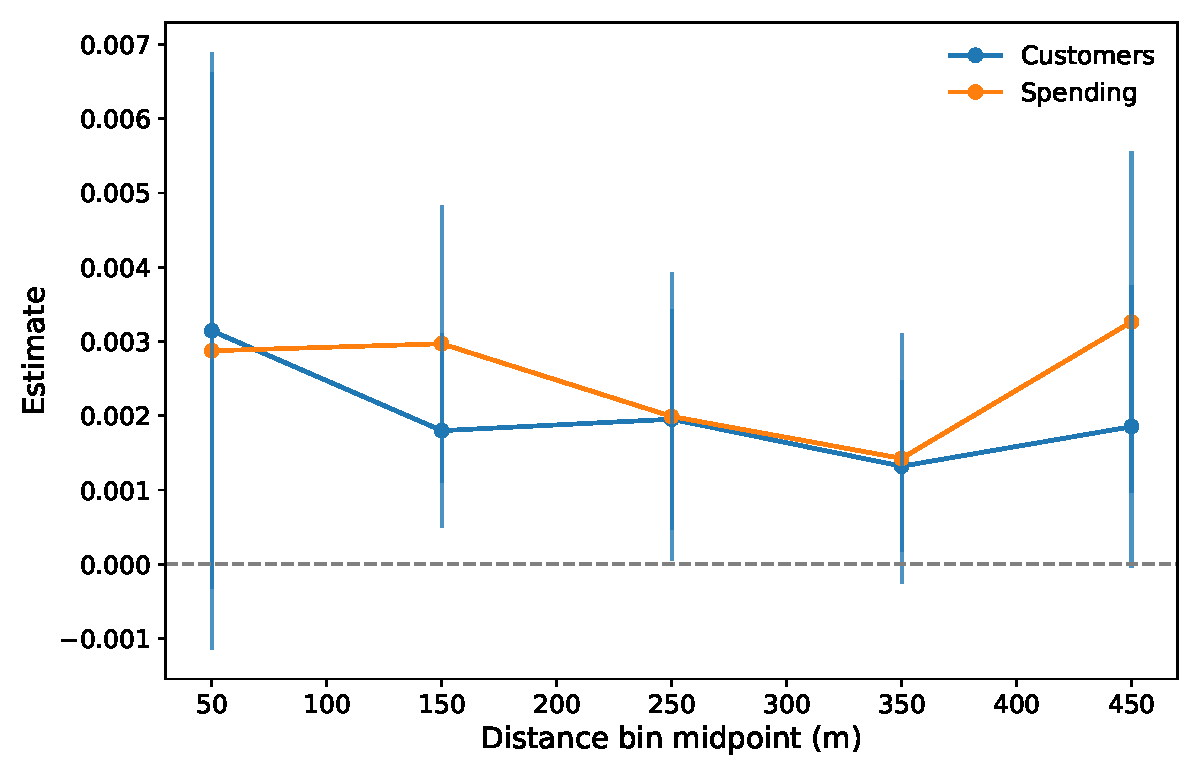
\includegraphics[width=\linewidth]{figures/narrow/02_distance_Period1_2019_All.pdf}
        \caption{2019}
    \end{subfigure}
    \hfill
    \begin{subfigure}{0.48\linewidth}
        \centering
        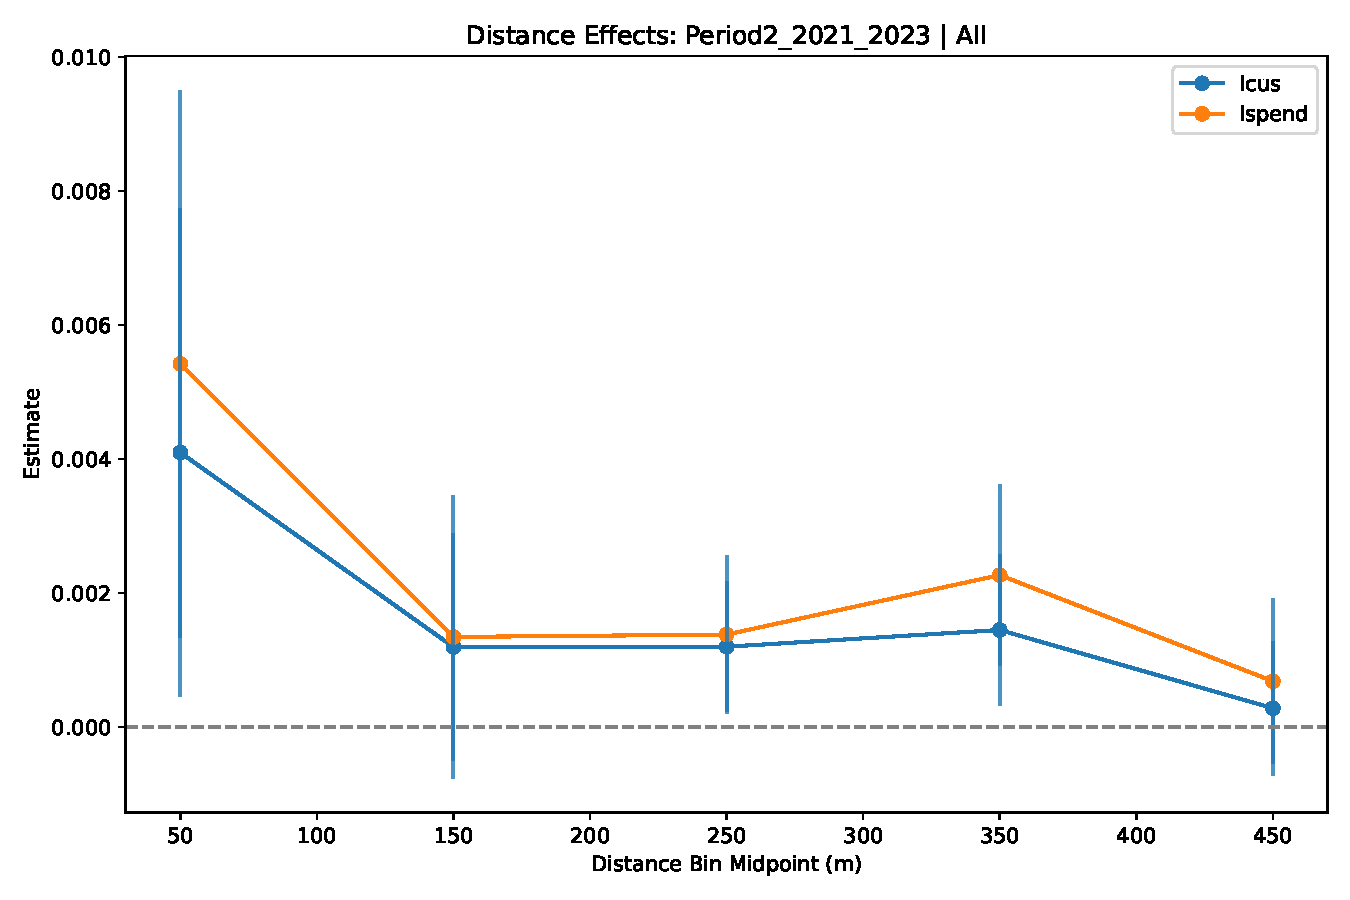
\includegraphics[width=\linewidth]{figures/narrow/02_distance_Period2_2021_2023_All.pdf}
        \caption{2021--2023}
    \end{subfigure}
    \caption{Narrow replication distance patterns for all POIs.}
    \label{fig:narrow-distance}
\end{figure}

\begin{figure}[!htbp]
    \centering
    \begin{subfigure}{0.48\linewidth}
        \centering
        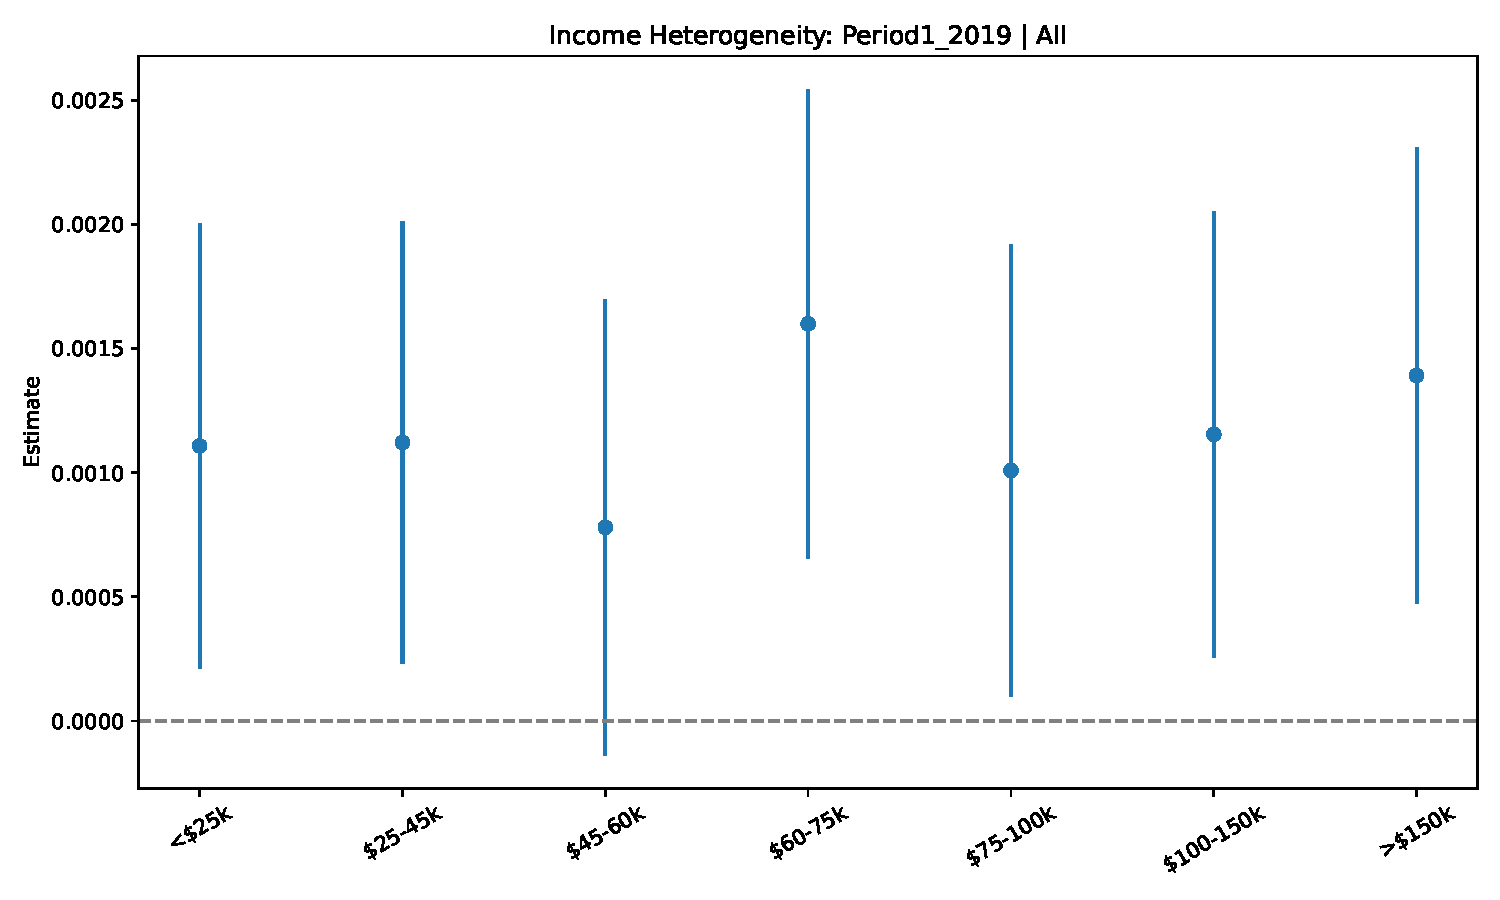
\includegraphics[width=\linewidth]{figures/narrow/04_income_Period1_2019_All.pdf}
        \caption{2019}
    \end{subfigure}
    \hfill
    \begin{subfigure}{0.48\linewidth}
        \centering
        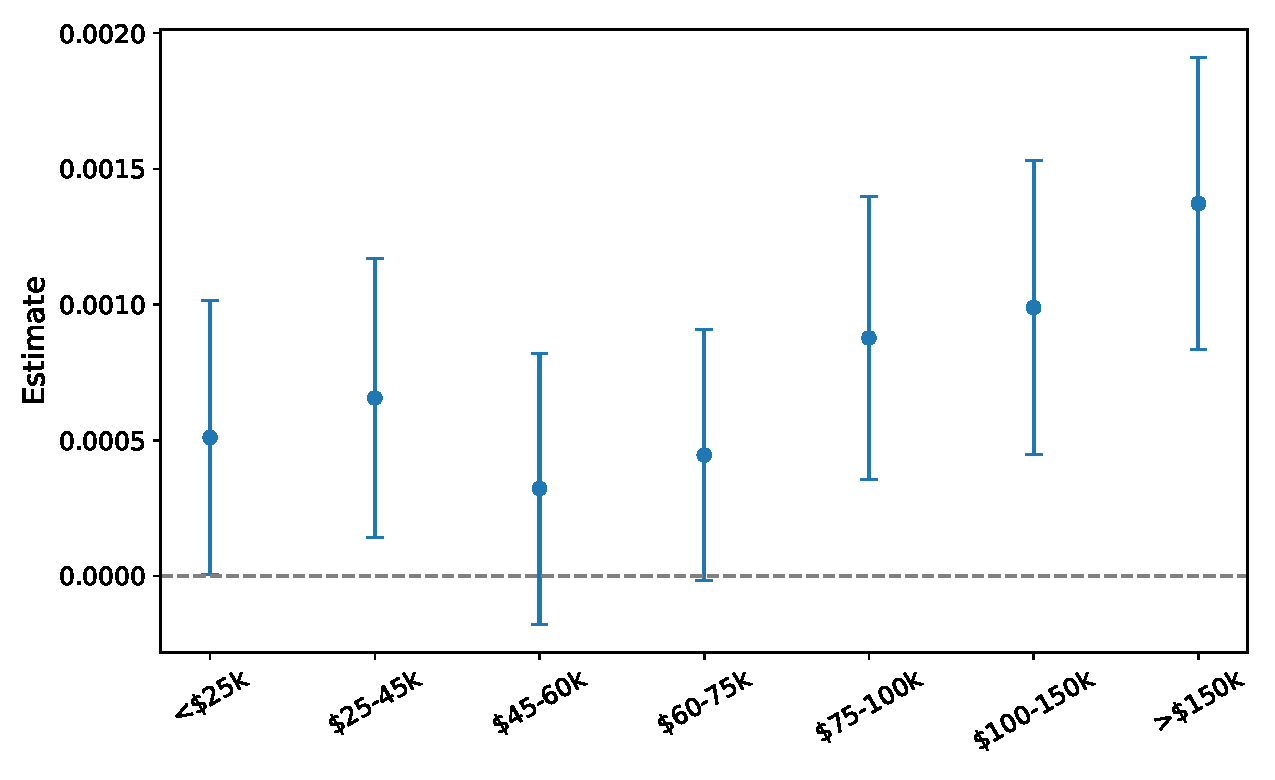
\includegraphics[width=\linewidth]{figures/narrow/04_income_Period2_2021_2023_All.pdf}
        \caption{2021--2023}
    \end{subfigure}
    \caption{Narrow replication income heterogeneity patterns for all POIs.}
    \label{fig:narrow-income}
\end{figure}

\begin{figure}[!htbp]
    \centering
    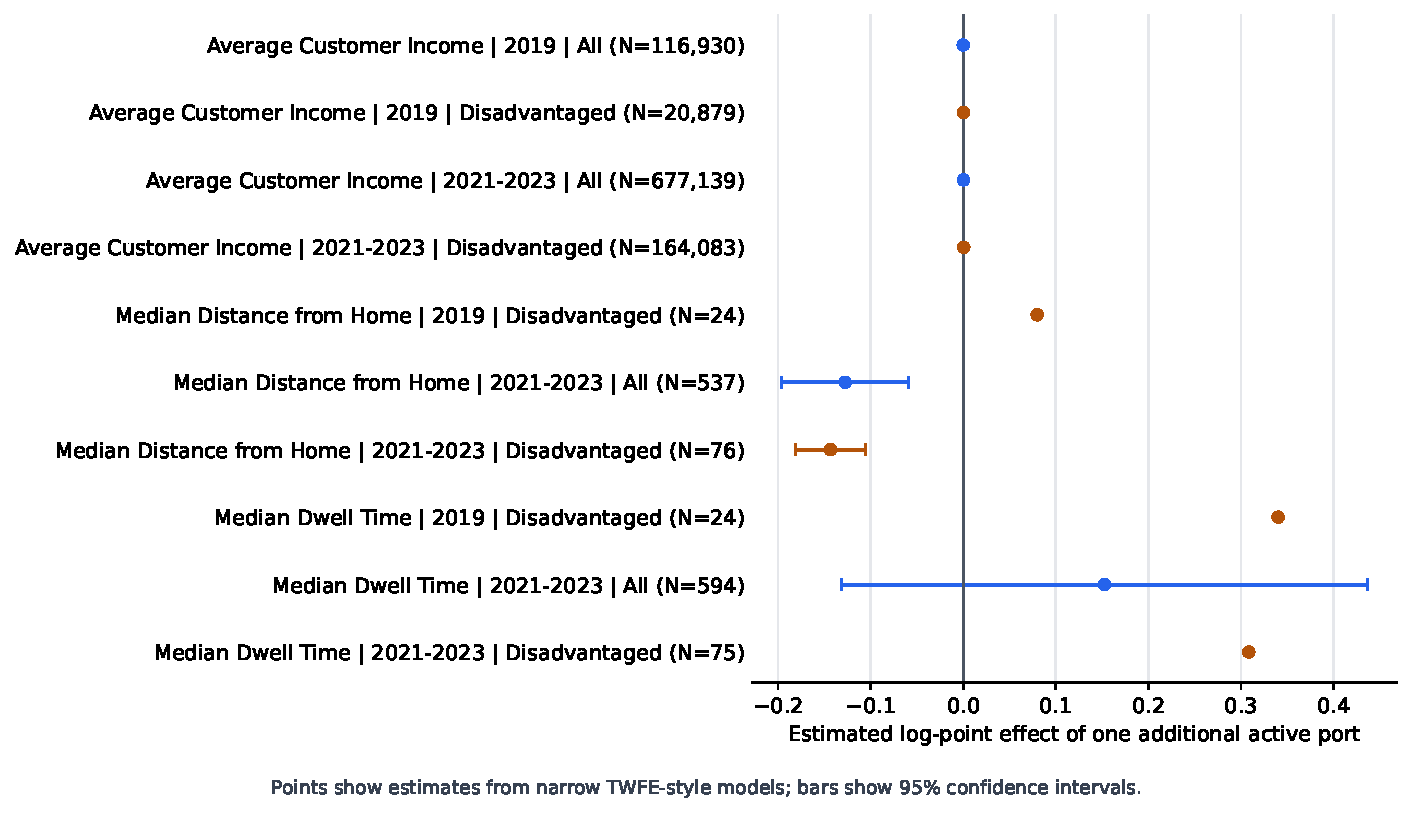
\includegraphics[width=0.95\linewidth]{figures/narrow/05_other_outcomes.pdf}
    \caption{Narrow replication auxiliary outcome effects.}
    \label{fig:narrow-other-outcomes}
\end{figure}

\FloatBarrier

\section{Broad Replication Results}

The Callaway-Sant'Anna (CS) staggered timing estimates would be preferred to the original TWFE models proposed in the original paper. However, these estimates underperform in this context. Since the CS estimators are attempting to recover effects from a noisy, extended study window with sparse treated units, the variance nullifies any effect identification. Additionally, the CS estimators function only with binary treatment. The EVCS installation includes several modifiers to treatment intensity (port count, charger type, etc.) which adds additional complexity that cannot be accounted for in binary treatment. 

Alternatively, the estimators for continuous treatment proposed by Callaway, Goodman-Bacon, and Sant'anna (insert reference) could be used in this setting as well. We selected a stacked regression model in this case as it can prevent "forbidden comparisons" of already-treated and not-yet-treated without limiting the statistical power of the model. This own-port model estimates a small negative all-port association for customer counts, a marginally negative all-port association for spending, and clearer negative associations for DC fast port exposure. Level 2 exposure is close to zero in the stacked specification. These results differ from the narrow TWFE estimates because the broader design uses a longer window, staggered timing, and in the case of the CS estimators, a different treatment estimand.

\begin{table}[!htbp]
\centering
\caption{Table 3. Broad replication estimates}
\begin{tabular}{lllllll}
\toprule
Model & Term & Outcome & Estimate (SE), \% & 95\% CI, \% & p & N \\
\midrule
CS timing & ATT & Customers & -0.690 (7.325) & [-13.972, 14.642] &  &  \\
CS timing & ATT & Spending & 3.023 (8.766) & [-13.241, 22.336] &  &  \\
Stacked own-port & All ports & Customers & -0.060*** (0.017) & [-0.094, -0.027] & < .001 & 8,796,470 \\
Stacked own-port & Level 2 ports & Customers & -0.026 (0.025) & [-0.075, 0.023] & .297 & 8,796,470 \\
Stacked own-port & DC fast ports & Customers & -0.105*** (0.023) & [-0.149, -0.060] & < .001 & 8,796,470 \\
Stacked own-port & All ports & Spending & -0.067** (0.022) & [-0.110, -0.025] & .002 & 8,796,470 \\
Stacked own-port & Level 2 ports & Spending & -0.051 (0.032) & [-0.113, 0.011] & .110 & 8,796,470 \\
Stacked own-port & DC fast ports & Spending & -0.088** (0.030) & [-0.146, -0.030] & .003 & 8,796,470 \\
\bottomrule
\end{tabular}
\begin{minipage}{0.95\linewidth}\footnotesize\emph{Note.} CS estimates are binary timing ATT estimates. Stacked estimates use a 6-month pre-window, 12-month post-window, stack-specific POI and county-month fixed effects, and POI-clustered standard errors.\end{minipage}
\end{table}


\begin{figure}[!t]
    \centering
    \begin{subfigure}{0.48\linewidth}
        \centering
        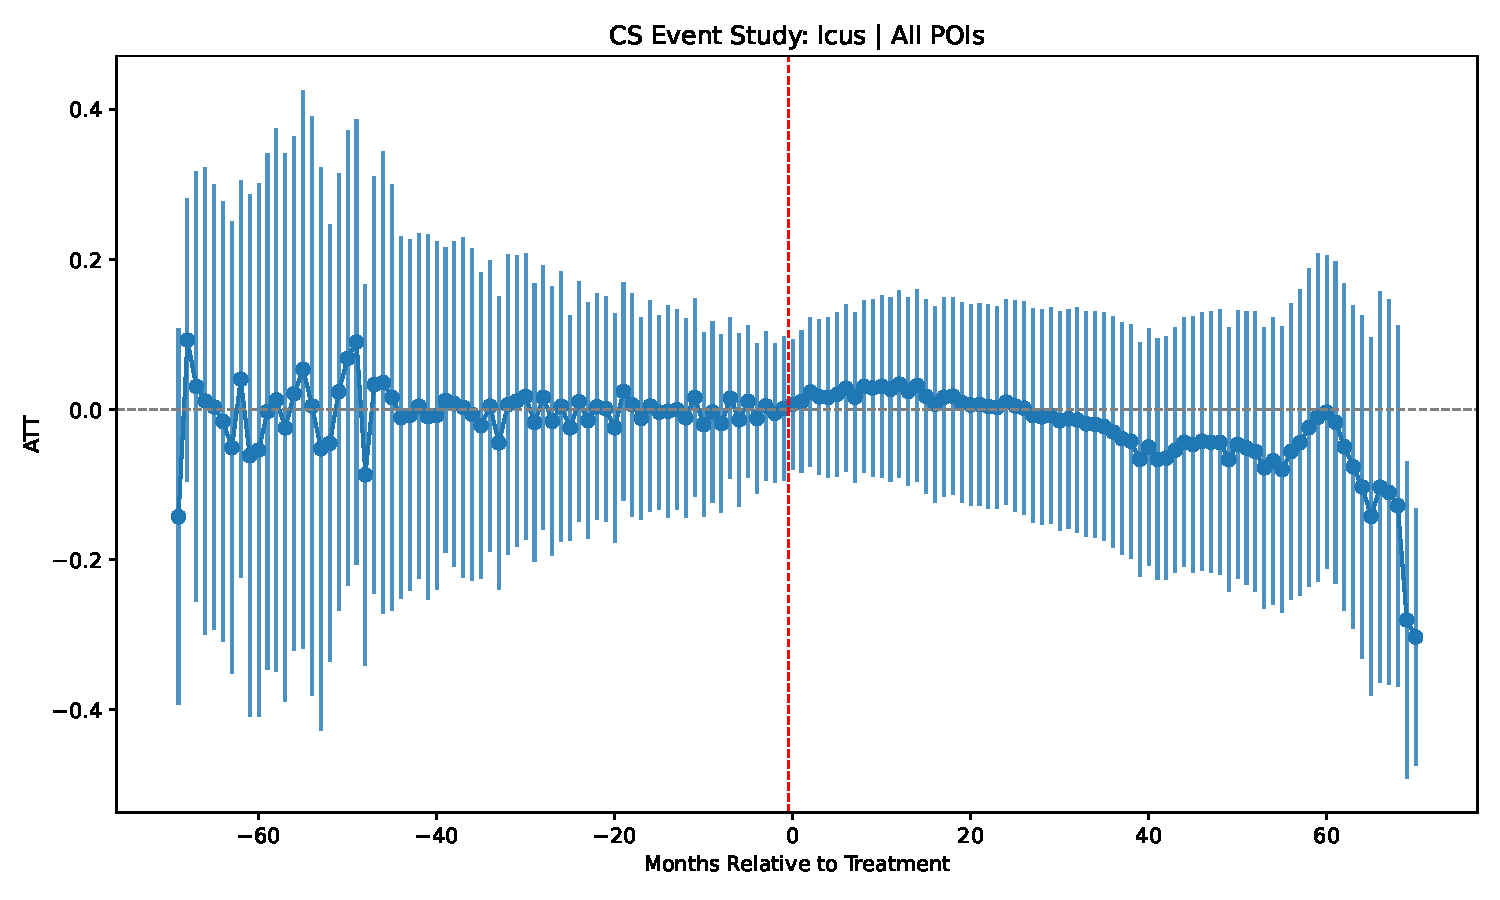
\includegraphics[width=\linewidth]{figures/broad/cs_event_study_All_POIs_lcus.pdf}
        \caption{Customers}
    \end{subfigure}
    \hfill
    \begin{subfigure}{0.48\linewidth}
        \centering
        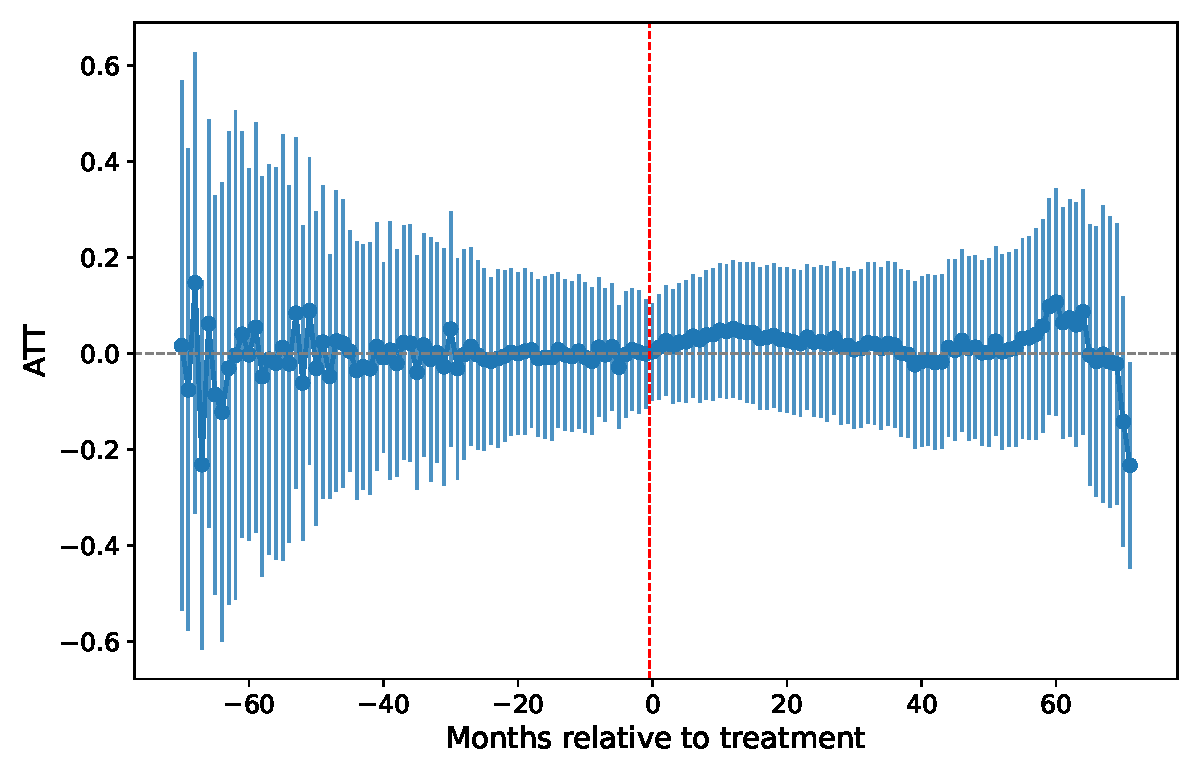
\includegraphics[width=\linewidth]{figures/broad/cs_event_study_All_POIs_lspend.pdf}
        \caption{Spending}
    \end{subfigure}
    \caption{Broad Callaway-Sant'Anna event-study diagnostics for all POIs.}
    \label{fig:broad-cs}
\end{figure}

\FloatBarrier

\section{Spatial Competition Extension}

The spatial competition design focuses on businesses outside the effective radius of an EVCS. Treatment in this context is defined as EVCS exposure at nearby same-sector competitors. Looking at same POI-type businesses with a 1km radius, all-port and Level 2 competitor exposure are essentially zero. However, DC fast competitor-port exposure is negative and statistically significant for both customers and spending.

Analysis of the monetary impact of these effects implies that DC fast competitor exposure is associated with about \$322 lower annual spending per affected competitor POI and about \$12.87 million lower annual spending across treated competitor POIs in the stacked regression spatial sample. The all-port and Level 2 monetary estimates have the opposite sign, but they are not statistically significant and should not be interpreted as evidence of positive spatial spillovers.

POI-type heterogeneity does not isolate a single sector as the clear source of the spatial competition pattern. Earlier versions of the analysis suggested restaurant-specific effects, but the updated estimates no longer support that interpretation. The sector results should therefore be treated as exploratory evidence on where the average DC fast competitor association may be concentrated, rather than as a separate restaurant mechanism.

\input{tables/table_04_spatial_stacked_main}

\begin{table}[!htbp]
\centering
\caption{Table 5. Monetary interpretation of spatial competition estimates}
\begin{tabular}{llll}
\toprule
Effect & Annual spend per competitor POI & Aggregate annual spend & Interpretation \\
\midrule
All competitor ports & \$7 & \$291,735 & Not statistically significant \\
DC fast competitor ports & -\$322 & -\$12,874,242 & Preferred monetary interpretation \\
Level 2 competitor ports & \$95 & \$3,817,351 & Not statistically significant \\
\bottomrule
\end{tabular}
\begin{minipage}{0.95\linewidth}\footnotesize\emph{Note.} Dollar values apply current stacked spatial spend coefficients to average active competitor-port exposure and baseline monthly spending among spatially treated focal competitor POIs.\end{minipage}
\end{table}


\begin{table}[!htbp]
\centering
\caption{Table 7. Spatial competition POI-type heterogeneity}
\begin{tabular}{lllll}
\toprule
POI type & Term & Outcome & Estimate (SE), \% & p \\
\midrule
Arts Entertainment & All competitor ports & Customers & 0.019 (0.023) & .409 \\
Arts Entertainment & DC fast competitor ports & Customers & -0.037 (0.055) & .504 \\
Arts Entertainment & All competitor ports & Spending & 0.032 (0.024) & .188 \\
Arts Entertainment & DC fast competitor ports & Spending & 0.006 (0.066) & .931 \\
Clothing & All competitor ports & Customers & 0.001* (0.001) & .033 \\
Clothing & DC fast competitor ports & Customers & -0.009 (0.011) & .421 \\
Clothing & All competitor ports & Spending & 0.001 (0.001) & .134 \\
Clothing & DC fast competitor ports & Spending & -0.008 (0.014) & .560 \\
Gas Convenience & All competitor ports & Customers & 0.025 (0.036) & .476 \\
Gas Convenience & DC fast competitor ports & Customers & -0.041 (0.054) & .456 \\
Gas Convenience & All competitor ports & Spending & 0.023 (0.046) & .611 \\
Gas Convenience & DC fast competitor ports & Spending & -0.028 (0.077) & .711 \\
Grocery & All competitor ports & Customers & -0.020 (0.021) & .360 \\
Grocery & DC fast competitor ports & Customers & 0.018 (0.029) & .531 \\
Grocery & All competitor ports & Spending & -0.017 (0.032) & .601 \\
Grocery & DC fast competitor ports & Spending & 0.025 (0.048) & .599 \\
Hotels & All competitor ports & Customers & 0.004 (0.075) & .960 \\
Hotels & DC fast competitor ports & Customers & -0.021 (0.085) & .804 \\
Hotels & All competitor ports & Spending & -0.116 (0.256) & .651 \\
Hotels & DC fast competitor ports & Spending & 0.163 (0.197) & .406 \\
Restaurants & All competitor ports & Customers & -0.001 (0.001) & .319 \\
Restaurants & DC fast competitor ports & Customers & -0.003 (0.002) & .084 \\
Restaurants & All competitor ports & Spending & -0.001 (0.002) & .536 \\
Restaurants & DC fast competitor ports & Spending & -0.003 (0.002) & .151 \\
Retail Other & All competitor ports & Customers & -0.011 (0.011) & .318 \\
Retail Other & DC fast competitor ports & Customers & -0.018 (0.015) & .232 \\
Retail Other & All competitor ports & Spending & -0.017 (0.015) & .272 \\
Retail Other & DC fast competitor ports & Spending & -0.008 (0.026) & .750 \\
\bottomrule
\end{tabular}
\begin{minipage}{0.95\linewidth}\footnotesize\emph{Note.} POI-type heterogeneity is estimated using the preferred stacked spatial competition design. The updated estimates do not isolate a single POI type as the clear source of the average DC fast competitor association.\end{minipage}
\end{table}


\section{Conclusion}

The narrow TWFE replication closely mirrors the original findings of this paper, supporting a positive relationship between EVCS exposure and nearby business activity in the original study time periods. However, after adding additional time periods and utilizing models that prevent "forbidden comparisons" of already-treated and not-yet-treated units, the staggered adoption and stacked regression estimates alter the interpretation. The broad stacked estimates no longer support a uniformly positive relationship between EVCS exposure and nearby activity. Instead, the clearest negative own-port associations appear for DC fast charging exposure, while Level 2 effects are close to zero and all-port spending is only marginally significant. The spatial competition extension also points to modest but economically meaningful losses from DC fast competitor exposure, with essentially null estimates for all competitor ports and Level 2 competitor ports.

The combined evidence demonstrates consistent narrow-window replication while showing that empirical design choices matter for interpretation. Given the pretrend diagnostics, the broad and spatial associations suggest that a simple mechanism of causal economic improvement may be incomplete in a wider study window.

\appendix

\FloatBarrier

\section{Appendix: Robustness and Diagnostics}

The stacked regression model robustness checks vary event windows, control unit limits, effect radii, and POI-category heterogeneity. After the battery, the main robust patterns are the negative DC fast own-port effects in the broad replication and negative DC fast competitor-port effects in the spatial competition extension. The updated POI-category heterogeneity estimates do not provide a stable restaurant-specific interpretation.

The pretrend and placebo diagnostics add important interpretative context. Significant pre-period terms indicate residual timing-pattern differences, so the stacked estimates should be framed as robust associations rather than definitive causal effects. Additional robustness checks and alternative model designs (CGBS) will be implemented to control for pretrend variance to solidify inference at a future date.

\begin{table}[!htbp]
\centering
\caption{Table 6. Spatial competition radius robustness}
\begin{tabular}{lllll}
\toprule
Radius & Term & Outcome & Estimate (SE), \% & p \\
\midrule
1000m & All competitor ports & Customers & 0.000 (0.001) & .980 \\
1000m & DC fast competitor ports & Customers & -0.007*** (0.002) & < .001 \\
1000m & All competitor ports & Spending & 0.000 (0.001) & .945 \\
1000m & DC fast competitor ports & Spending & -0.005* (0.002) & .011 \\
1500m & All competitor ports & Customers & -0.005*** (0.001) & < .001 \\
1500m & DC fast competitor ports & Customers & -0.007*** (0.001) & < .001 \\
1500m & All competitor ports & Spending & -0.004*** (0.001) & < .001 \\
1500m & DC fast competitor ports & Spending & -0.005*** (0.001) & < .001 \\
2000m & All competitor ports & Customers & -0.006*** (0.001) & < .001 \\
2000m & DC fast competitor ports & Customers & -0.008*** (0.001) & < .001 \\
2000m & All competitor ports & Spending & -0.005*** (0.001) & < .001 \\
2000m & DC fast competitor ports & Spending & -0.007*** (0.001) & < .001 \\
\bottomrule
\end{tabular}
\begin{minipage}{0.95\linewidth}\footnotesize\emph{Note.} Radius robustness uses the stacked spatial competition estimator at competition radii above the 500m direct-treatment radius.\end{minipage}
\end{table}


\begin{table}[!htbp]
\centering
\caption{Table 8. Stacked pretrend and placebo diagnostics}
\begin{tabular}{llllll}
\toprule
Target & Outcome & Term & Estimate & SE & p \\
\midrule
Broad & Customers & treated lead m6 & 0.0130*** & 0.0033 & < .001 \\
Broad & Customers & treated lead m5 & 0.0134*** & 0.0032 & < .001 \\
Broad & Customers & treated lead m4 & 0.0050 & 0.0030 & .098 \\
Broad & Customers & treated lead m3 & 0.0003 & 0.0028 & .920 \\
Broad & Customers & treated lead m2 & -0.0014 & 0.0025 & .571 \\
Broad & Customers & placebo treated last3 pre months & -0.0108*** & 0.0021 & < .001 \\
Broad & Spending & treated lead m6 & 0.0228*** & 0.0048 & < .001 \\
Broad & Spending & treated lead m5 & 0.0193*** & 0.0047 & < .001 \\
Broad & Spending & treated lead m4 & 0.0116* & 0.0046 & .011 \\
Broad & Spending & treated lead m3 & 0.0004 & 0.0044 & .933 \\
Broad & Spending & treated lead m2 & 0.0002 & 0.0041 & .968 \\
Broad & Spending & placebo treated last3 pre months & -0.0176*** & 0.0030 & < .001 \\
Spatial & Customers & treated lead m6 & 0.0152*** & 0.0045 & < .001 \\
Spatial & Customers & treated lead m5 & 0.0088* & 0.0044 & .045 \\
Spatial & Customers & treated lead m4 & 0.0024 & 0.0041 & .567 \\
Spatial & Customers & treated lead m3 & -0.0017 & 0.0038 & .648 \\
Spatial & Customers & treated lead m2 & 0.0001 & 0.0034 & .983 \\
Spatial & Customers & placebo treated last3 pre months & -0.0093** & 0.0029 & .001 \\
Spatial & Spending & treated lead m6 & 0.0155* & 0.0067 & .021 \\
Spatial & Spending & treated lead m5 & 0.0060 & 0.0066 & .364 \\
Spatial & Spending & treated lead m4 & 0.0003 & 0.0063 & .964 \\
Spatial & Spending & treated lead m3 & -0.0017 & 0.0060 & .772 \\
Spatial & Spending & treated lead m2 & -0.0021 & 0.0055 & .701 \\
Spatial & Spending & placebo treated last3 pre months & -0.0084* & 0.0041 & .042 \\
\bottomrule
\end{tabular}
\begin{minipage}{0.95\linewidth}\footnotesize\emph{Note.} Significant pre-period terms indicate residual timing-pattern differences. These diagnostics motivate cautious causal language for stacked estimates.\end{minipage}
\end{table}


\FloatBarrier

\section{Appendix Roadmap}

Data access and reproducibility details are documented in \texttt{docs/data\_access.md} and \\ \texttt{docs/reproduction.md}. The model hierarchy is documented in \texttt{docs/model\_architecture.md}. Deferred improvements are listed in \texttt{docs/future\_work.md}.

Additional appendix material can include narrow distance, charger-type, income, and other-outcome tables; stacked window and control-cap robustness tables; stacked spatial radius and POI-type robustness tables; and exploratory broad and spatial intensity diagnostics. The numerical source of truth is \texttt{output/tables/}; APA-style manuscript tables are stored in \texttt{paper/tables/}.

\end{document}
